% chapitre de connexion et de création d'un compte
\chapter{Se connecter à ou créer son compte}
%\addcontentsline{toc}{chapter}{Se connecter à ou créer son compte}

\section{La première connexion}
La première chose à faire est de se connecter au site du portail qui est situé à \url{https://portail.apps.education.fr} comme le montre la capture d'écran suivante~:
\begin{figure}
    \centering
    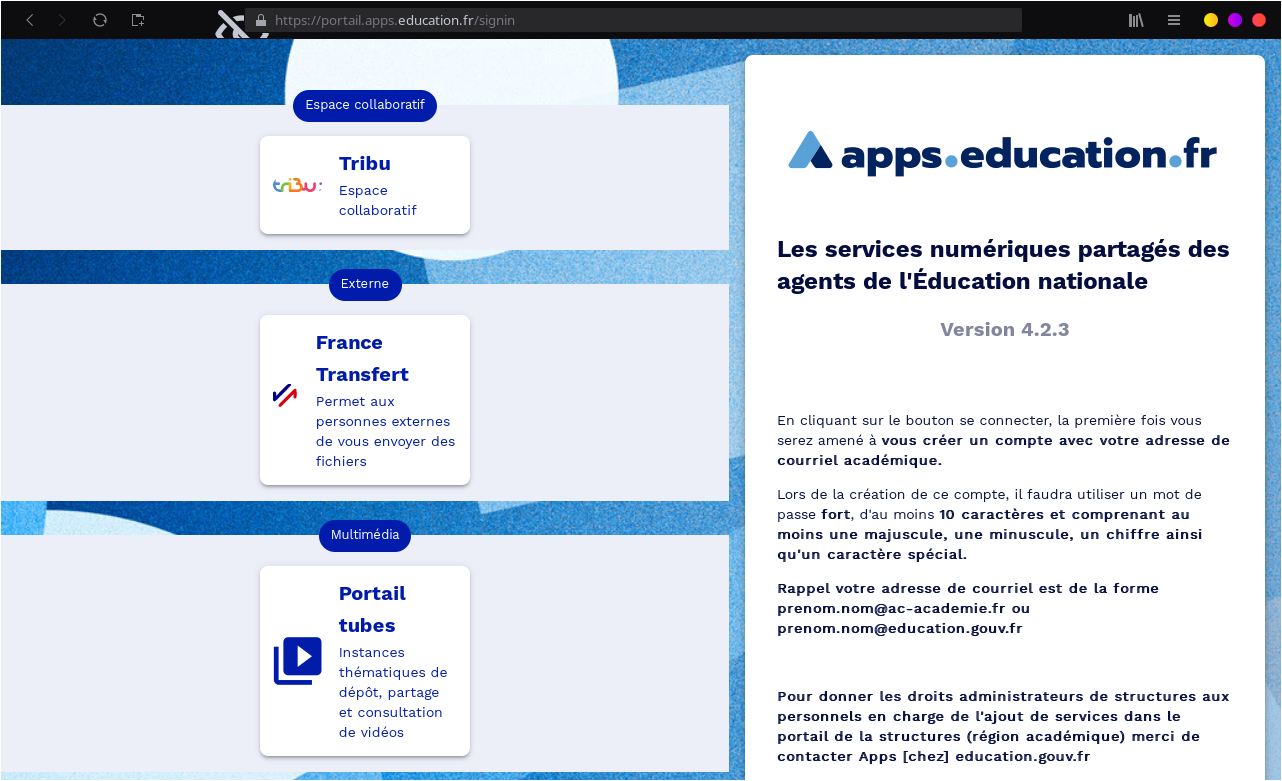
\includegraphics[width=0.7071\linewidth]{Captures/portail.site.web.png}
\end{figure}

En bas à gauche se trouve le bouton \fbox{\hspace{1cm}SE~CONNECTER\hspace{1cm}} il donne alors accès à la fenêtre de connexion qui suit. 
\begin{figure}
	\centering
	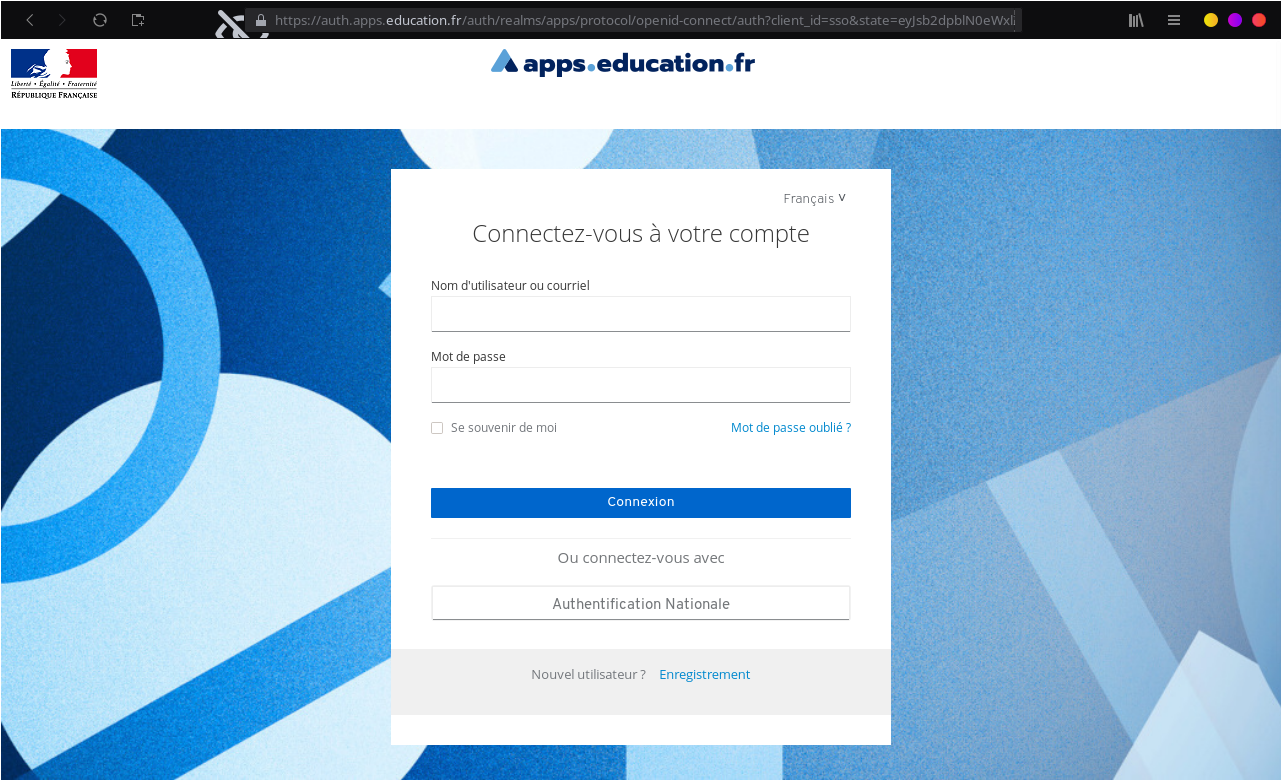
\includegraphics{./Captures/portail.site.web.connexion.png}
\end{figure}

Si on y regarde de plus près, on voit qu'on peut s'y connecter en saisissant son adresse professionnelle (académique ou ministérielle) mais également via un nom d'utilisateur. 
\begin{figure}
	\centering
	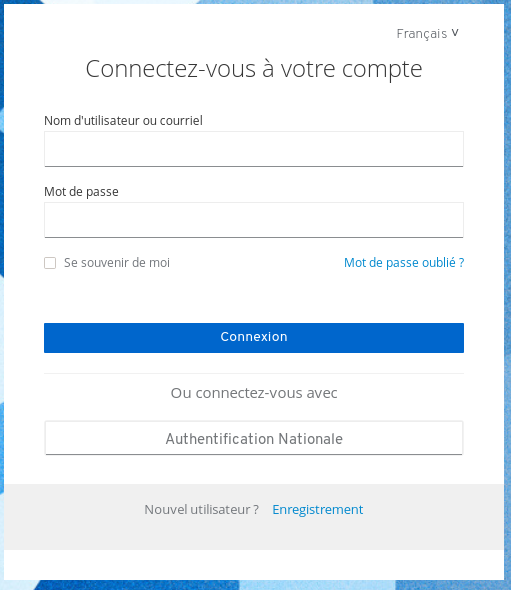
\includegraphics[width=0.500\linewidth]{./Captures/portail.site.web.connexion.zoom.png}
\end{figure}
Vers le bas de la fenêtre, une connexion avec ``Authentification Nationale'' est proposée, cette authentification sera abordée dans un \emph{attendum} ultérieur.

Évidemment la première fois impossible d'utiliser cette fenêtre de connxion puisque ``La Boîte'' ne nous connaît pas, aussi, la présence en bas à droite du lien \href{https://auth.apps.education.fr/auth/realms/apps/login-actions/registration}{Enregistrement} va permettre l'inscription au service et à compter de ce moment-là cette fenêtre de connexion suffira.

La fenêtre d'enregistrement, comme cette capture, montre la présence en quatrième ligne d'un champ dédié à l'identifiant, c'est là qu'il faudra l'inventer en suivant les règles demandées et précisées en dessous du chmap.
\begin{figure}
	\centering
	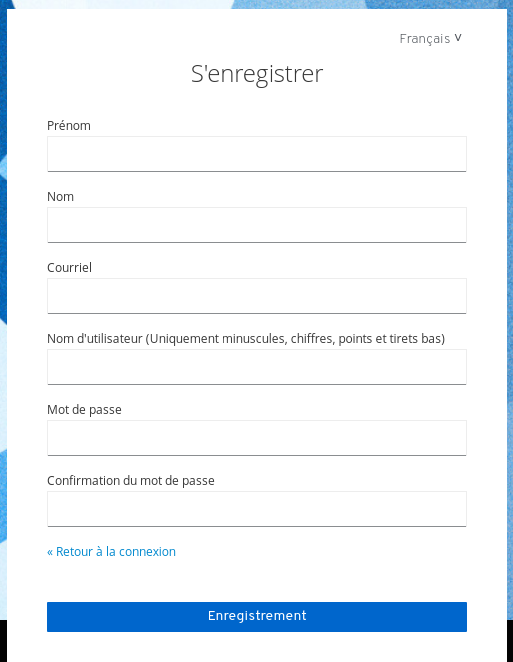
\includegraphics[width=0.500\linewidth]{./Captures/portail.site.web.enregistrement.png}
	\caption{}
\end{figure}

\paragraph{Avantage de l'identifiant.} Au cours d'une carrière nous sommes tous amenés à changer d'établissements, et une partie d'entre nous pour ne pas dire une majorité, nous changeons d'académie. 
Dès lors, le changement d'adresse mail s'opère pour chaque agent, et, comme l'intention de la boite est de rester un outil pérenne qui suit l'agent dans le temps, il faut pouvoir s'y connecter même en changeant de fonction ou d'académie, aussi la présence de cet identifiant vous permettra de vous connecter au compte et ensuite d'y modifier l'adresse mail de rattachement.

Une fois cette étape prête, un lien vers la fenêtre de confirmation sera envoyé à l'adresse de courriel précisée dans le formulaire précédent, soyez relativement rapides, ce lien arrive vite à expiration, je conseille d'ailleurs d'avoir ouvert sa messagerie avant la phase d'enregistrement pour s'assurer de la réception du lien par courriel et de l'activation au plus vite du profil.

\section{Derniers réglages du profil simplifié.}
Lors de la première connexion une fenêtre demande à l'utilisateur de bien vouloir mettre à jour son profil. 
C'est alors vers une version simplifiée de ces modifications qu'est dirigé l'utilisateur. 
Vous aurez remarqué qu'un lien 
\begin{figure} \label{fig-profil-haut}
	\centering
	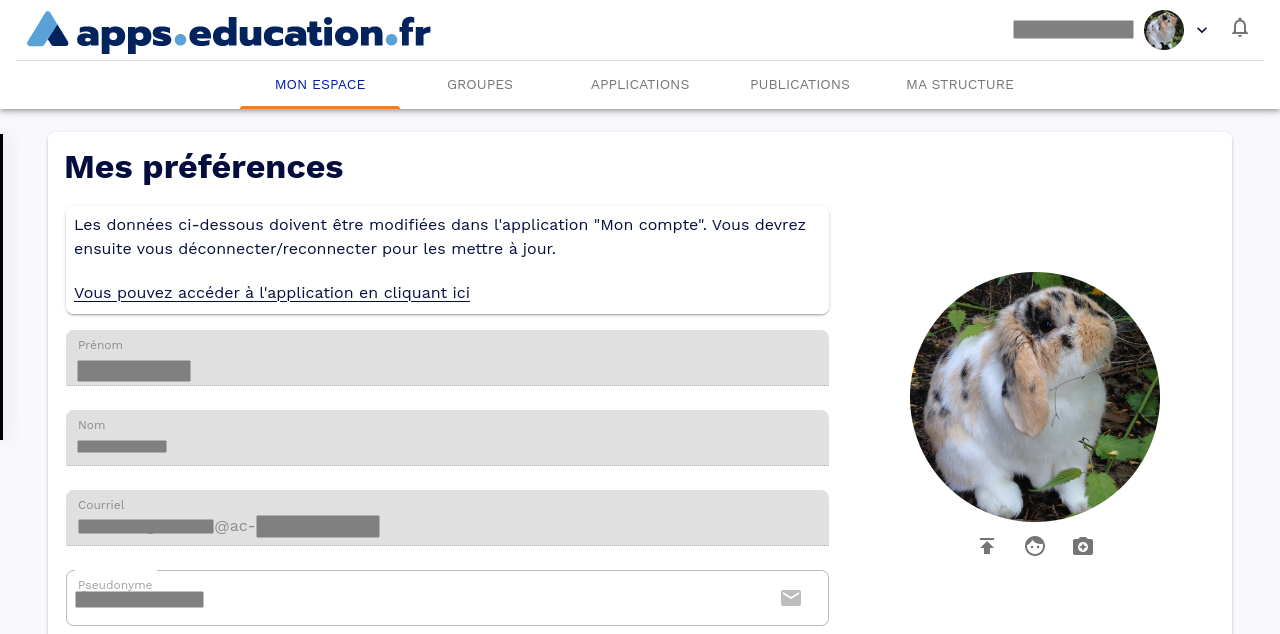
\includegraphics{./Captures/portail.profil.haut.png}
	\caption{Haut du profil simplifié}
\end{figure}
Vous aurez remarqué sur la figure \ref{fig-profil-haut} qu'un lien est présent au beau milieu du texte, avec le texte \emph{Vous pouvez accéder à l'application en cliquant ici}, donnant accès à la configuration plus avancée du profil et détaillée dans la sous-section \ref{ssec-profil-detail}. 
Sur cette partie de l'écran capturé, vous voyez que rien ne semble modifiable, mais apparaîtront vos Nom, prénom et adresse de courriel académique utilisés et déclarés pendant l'enregistrement.
\begin{figure}
	\centering
	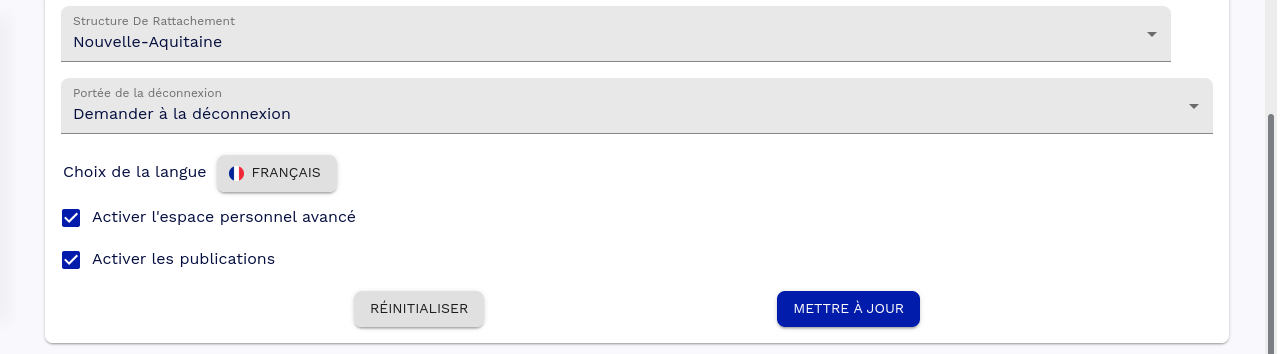
\includegraphics{./Captures/portail.profil.milieu.png}
	\caption{Partie centrale du profil}
\end{figure}
La partie centrale du profil contient elle des éléments de rattachement tant géographique qu'académique -- au sens région académique -- ainsi que des réglages sur la déconnexion du portail et le comportement auprès des autres applications en lien et intégrées avec ce dernier, mais aussi des réglages sur les publications qui ne manqueront pas d'être produite par l'utilisateur.
\begin{figure}
	\centering
	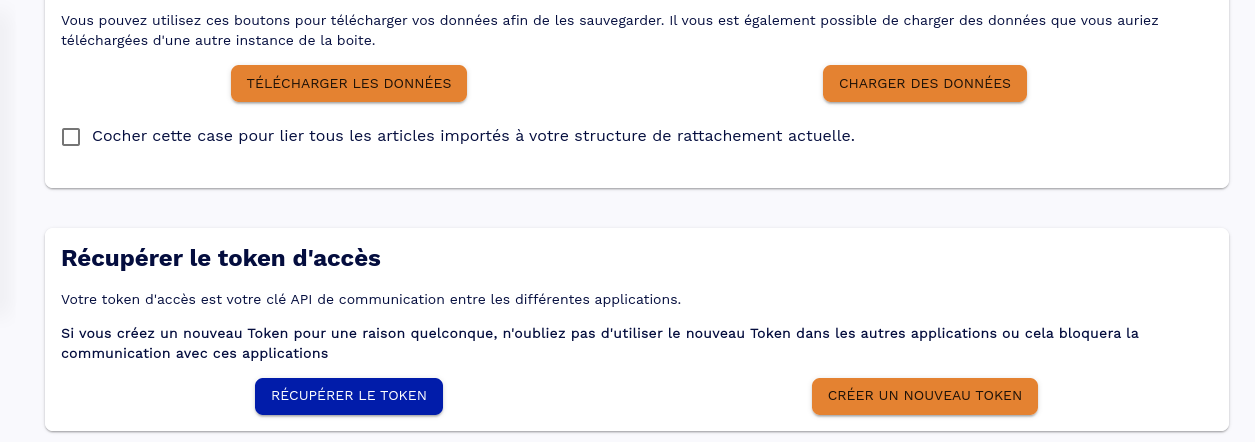
\includegraphics{./Captures/portail.profil.bas.png}
	\caption{}
\end{figure}
La partie inférieure du profil simplifié est liée aux données personnelles sauvegardables ou importables dans le profil, ce qui n'est pas forcément habituel sur de nombreuses plateformes, et pour finir un outil de génération de token pour développer des outils d'interconnexion avec ce profil.

N'étant pas familier avec ce dernier point, je n'ai pas insisté sur son utilisation, je me suis juste contenté de sauvegarder le contenu de cette clé.

\section{Réglages fins du profil et augmentation de la sécurité.} \label{ssec-profil-detail}
Il peut arriver d'avoir besoin de modifier des détails fournis lors de l'enregistrement. 
C'est alors sept parties différentes qui deviennent accessibles sur la plateforme \emph{keycloack} pour leur modification. 

Quand de tels changement peuvent-ils intervenir~? 
Voici un exemple simple. 
Un jour vous décidez et obtenez une mutation interacadémique, votre travail accumulé sur l'espace de stockage, vos vidéos pédagogiques et autres contenus multimédia dans les pod Educ ou encore le Tube, tout ceci étant initialement rattaché à votre adresse académique pourrait-il se perdre, d'autant que d'autres services viendront sûrement se lier à apps~?
La réponse est simple, il suffit de vous connecter à apps, grâce à l'identifiant qui lui restera toujours valide, puis, modifier les détails avancés, comme par exemple dans ce cas-là renseigner votre nouvelle adresse de courriel professionnel. 

Pour cela il suffira de vous connecter à votre portail, d'aller ensuite dans le menu du profil.
\begin{figure}
	\centering
	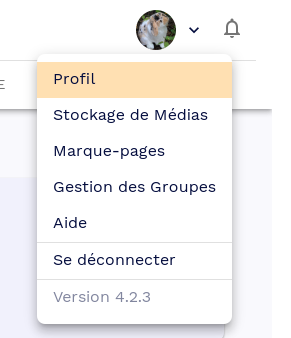
\includegraphics[width=0.3333\linewidth]{./Captures/menu.profil.png}
%	\caption{}
\end{figure}
Puis ensuite de cliquer sur le lien pour accéder à l'application par le lien \emph{Vous pouvez accéder à l'application en cliquant ici\/} et de là les différentes fenêtres suivante seront visibles, le choix s'effectuant par la partie gauche de la fenêtre faisant apparaître les différentes catégories.

\subsection{Modification des données personnelles}
Nom, prénom et adresse de courrier électronique se changent dans ce premier onglet, l'identifiant est quant à lui immuable, car c'est lui qui restera pérenne tout le long de l'utilisation de la plateforme et des années de son usage.
\begin{figure}
	\centering
	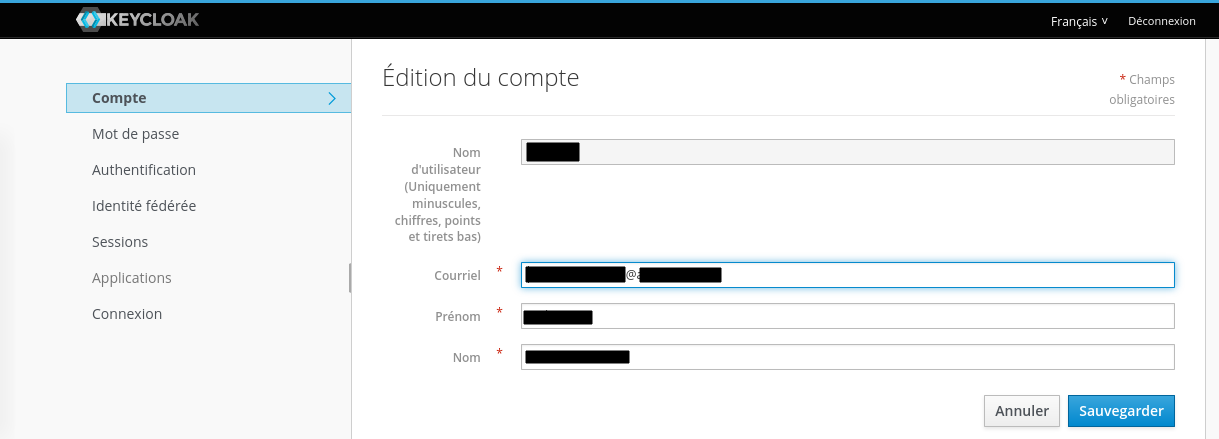
\includegraphics{./Captures/keycloack.profil.compte.png}
	\caption{Modification avancée du profil, paramètre de }
\end{figure}

\subsection{Modification du mot de passe}
C'est dans cet onglet que pourra être changé le mot de passe d'accès à tous les services, tous se synchroniseront à partir de lui.
\begin{figure}
	\centering
	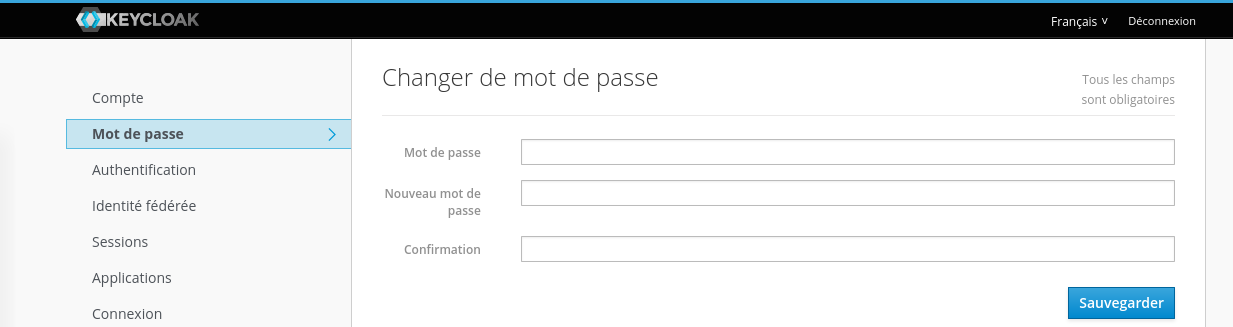
\includegraphics{./Captures/keycloack.profil.mdp.png}
	\caption{Modification avancée du profil, paramètre de }
\end{figure}

\subsection{Modification du mode d'authentification}
Par défaut, l'utilisation seule du mot de passe et de l'identifiant sont les deux informations pour assurer la sécurité de l'accès au compte utilisateur, mais il existe une méthode supplémentaire d'authentification par l'emploi de la méthode du \emph{One Time Password\/} ou OTP en installant sur \emph{smartphone} par exemple une application comme par exemple FreeOTP.
\begin{figure}
	\centering
	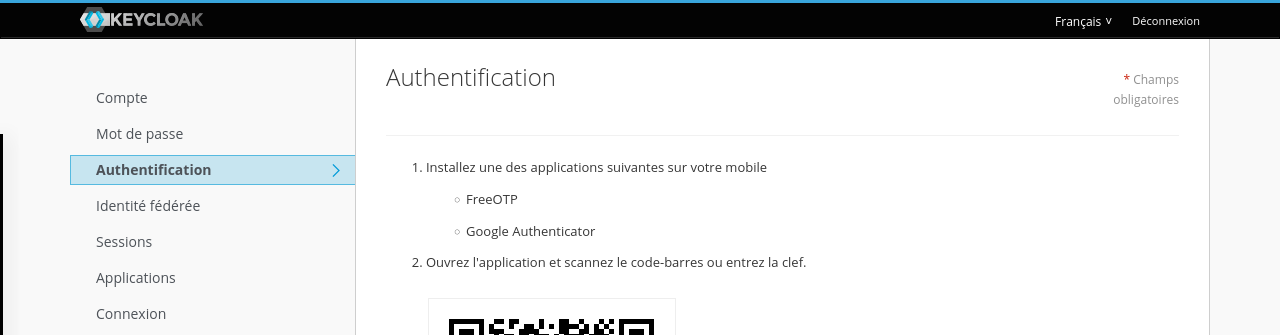
\includegraphics{./Captures/keycloack.profil.authentification.haut.png}
	\caption{Modification avancée du profil, paramètre de }
\end{figure}
Une telle application demande soit manuellement de saisir certaines informations relatives au secret partagé et à la méthode permettant de générer par la suite les mots de passe, soit plus simplement de flasher un QR-Code tel que l'affiche l'image qui suit.
\begin{figure}
	\centering
	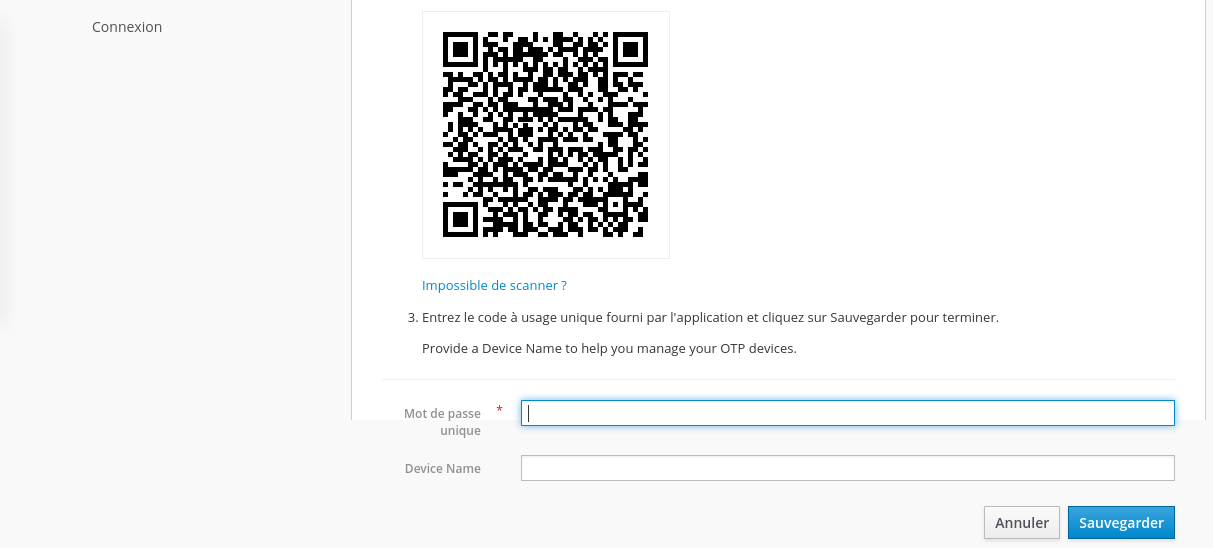
\includegraphics{./Captures/keycloack.profil.authentification.bas.png}
	\caption{Modification avancée du profil, paramètre de }
\end{figure}
Lors d'une connexion ultérieurs et après sauvegarde des paramètres par la saisie de la réponse dans la ligne adéquate, la figure suivante apparaîtra.
\begin{figure}
	\centering
	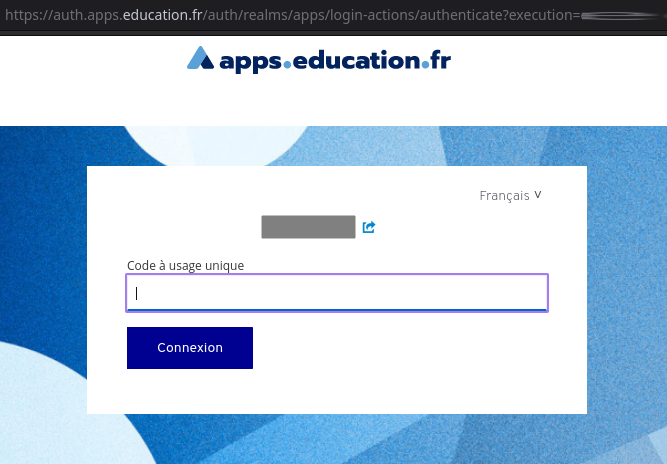
\includegraphics[width=0.500\linewidth]{./Captures/portail.otp.png}
	\caption{La sur-sécurité par OTP}
\end{figure}
\paragraph*{Petit conseil.} Ne perdez pas votre périphérique, voir, ce qui est possible sur FreeOTP+, partagez ce même QR-Code sur un deuxième dispositif (tablette, ...) pour le cas échéant si l'un des dispositifs vient à ne plus être disponible, pouvoir accéder au compte pour désactiver cette fonctionnalité.

\subsection{Modification et ajout d'identités en fédération}
\begin{figure}
	\centering
	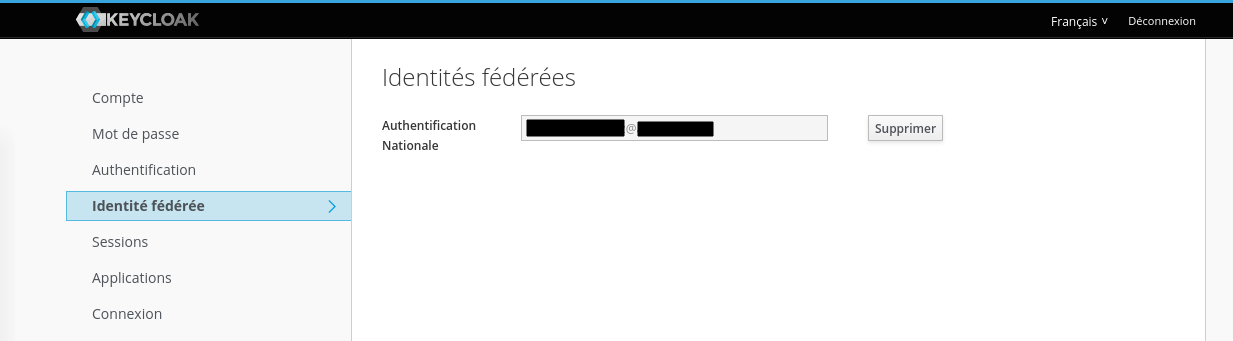
\includegraphics{./Captures/keycloack.profil.identite.federee.png}
	\caption{Modification avancée du profil, paramètre de }
\end{figure}

Passé ces premiers onglets où des informations sont altérables, les suivants ne sont plus qu'informatifs.

\subsection{Accès aux sessions}
Par cet onglet vous accéderez à l'information des sessions actuellement actives. 
Ici il n'y en a qu'une puisque seul un ordinateur avec une session est branché sur Apps.Education.
\begin{figure}
	\centering
	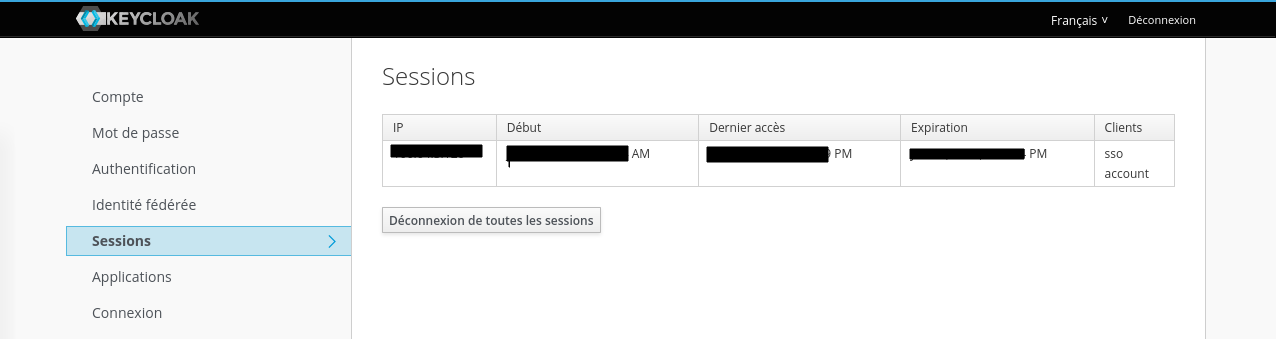
\includegraphics{./Captures/keycloack.profil.sessions.png}
	\caption{Les sessions en cours.}
\end{figure}

\subsection{Méthodes d'accès des applications.}
L'onglet suivant sert quant à lui à montrer les méthodes d'accès utilisées par les applications déjà utilisées ou en cours d'usage permettant aussi d'avoir un panoramique des accès qu'elles emploient pour communiquer avec les bases de données internes au projet (à vérifier).
\begin{figure}
	\centering
	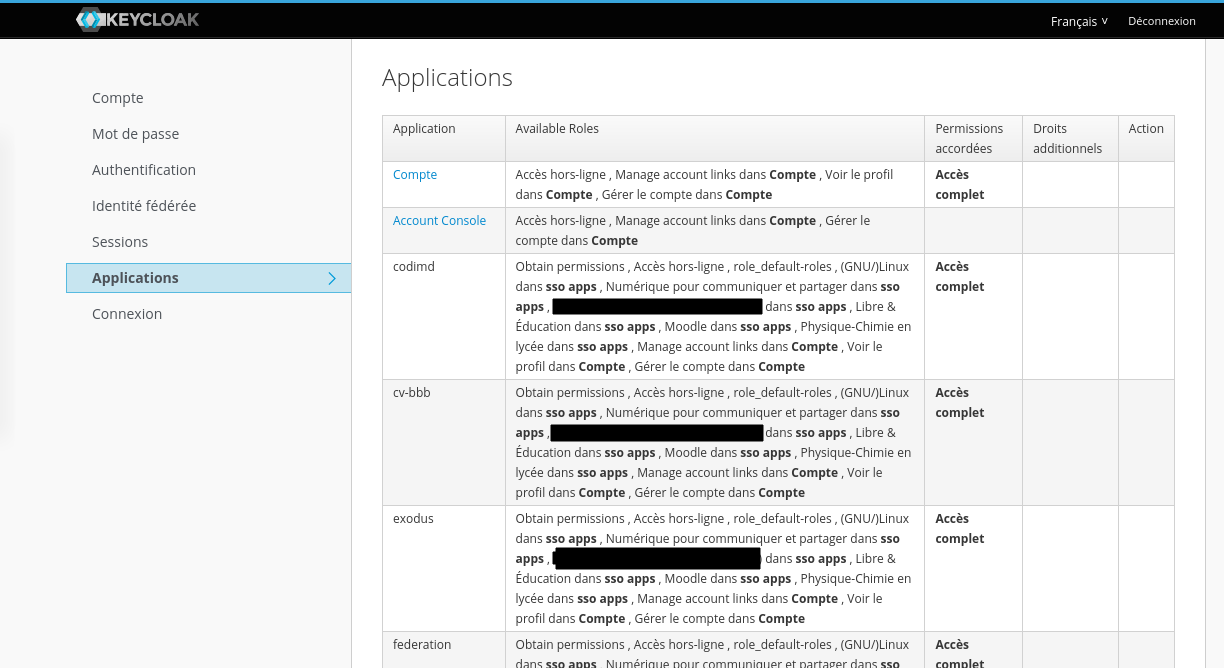
\includegraphics{./Captures/keycloack.profil.applications.png}
	\caption{Modification avancée du profil, paramètre de }
\end{figure}

\subsection{Les logs !}
\begin{figure}
	\centering
	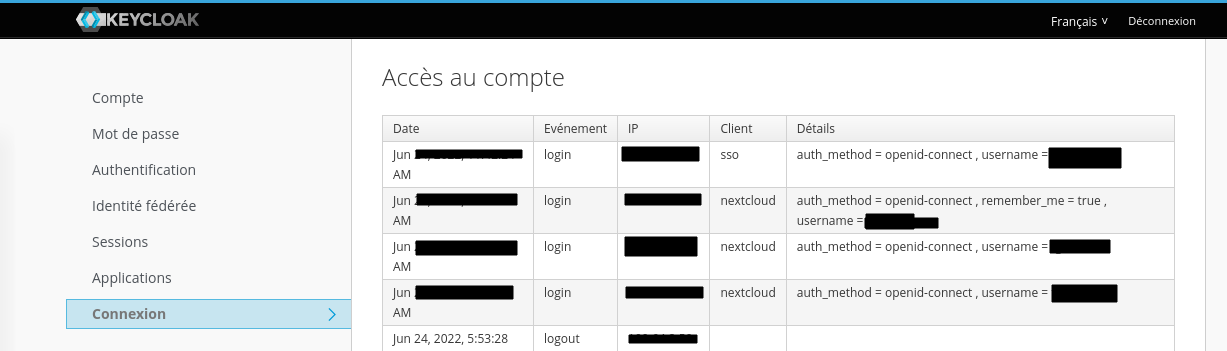
\includegraphics{./Captures/keycloack.profil.connexions.log.png}
	\caption{Modification avancée du profil, paramètre de }
\end{figure}